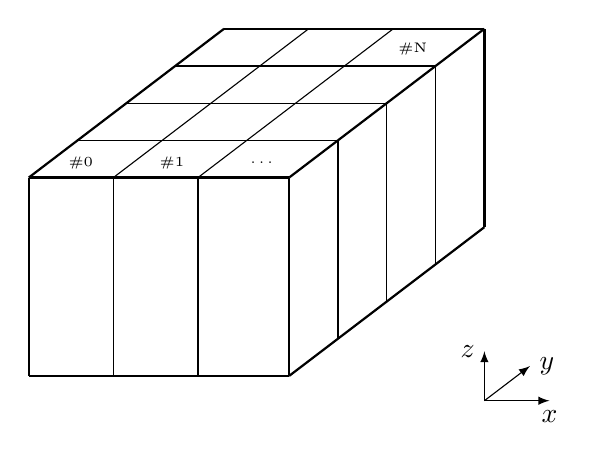
\begin{tikzpicture}[scale=1.4]
\begin{scope}[x={0 250},y={0 200}]
%        %% next four lines will help you to locate the point needed by forming a grid. comment these four lines in the final picture.↓
%        \draw[help lines,xstep=.1,ystep=.1] (0,0) grid (1,1);
%        \draw[help lines,xstep=.05,ystep=.05] (0,0) grid (1,1);
%        \foreach \x in {0,1,...,9} { \node [anchor=north] at (\x/10,0) {0.\x}; }
%        \foreach \y in {0,1,...,9} { \node [anchor=east] at (0,\y/10) {0.\y};}
%        %% upto here↑

% domain
\draw[thick] (0.1,0.1) -- (0.5,0.1);
\draw[thick] (0.1,0.1) -- (0.1,0.5);
\draw[thick] (0.1,0.5) -- (0.5,0.5);
\draw[thick] (0.5,0.1) -- (0.5,0.5);
\draw[thick] (0.5,0.1) -- (0.8,0.4);
\draw[thick] (0.5,0.5) -- (0.8,0.8);
\draw[thick] (0.8,0.4) -- (0.8,0.8);
\draw[thick] (0.1,0.5) -- (0.4,0.8);
\draw[thick] (0.4,0.8) -- (0.8,0.8);

% axis
\draw[-latex] (0.8,0.05) -- (0.9,0.05)node[anchor=north]{$x$};
\draw[-latex] (0.8,0.05) -- (0.8,0.15)node[anchor=east]{$z$};
\draw[-latex] (0.8,0.05) -- (0.87,0.12)node[anchor=west]{$y$};

% decomposition
\draw (0.23,0.1) -- (0.23,0.5);
\draw (0.36,0.1) -- (0.36,0.5);
\draw (0.53,0.8) -- (0.23,0.5);
\draw (0.66,0.8) -- (0.36,0.5);
\draw (0.575,0.175) -- (0.575,0.575);
\draw (0.65,0.25) -- (0.65,0.65);
\draw(0.725,0.325) -- (0.725,0.725);
\draw (0.175,0.575) -- (0.575,0.575);
\draw (0.25,0.65) -- (0.65,0.65);
\draw(0.325,0.725) -- (0.725,0.725);

% ranks
\draw (0.18,0.53)node[rotate=0]{\tiny{\#0}};
\draw (0.32,0.53)node[rotate=0]{\tiny{\#1}};
\draw (0.46,0.53)node[rotate=0]{\tiny{\dots}};
\draw (0.69,0.76)node[rotate=0]{\tiny{\#N}};


\end{scope}
\end{tikzpicture}
